A problem in finding and tracking a particle was that the surface of the PDMS was very uneven and sharp ridges along the length of the channel appeared as seen in Figure \ref{fig:unpolished} unless the focus was in a narrow depth of the channel. 
 
 \begin{figure}[H]
 \centering
 \begin{subfigure}[3a]{0.40\textwidth}
 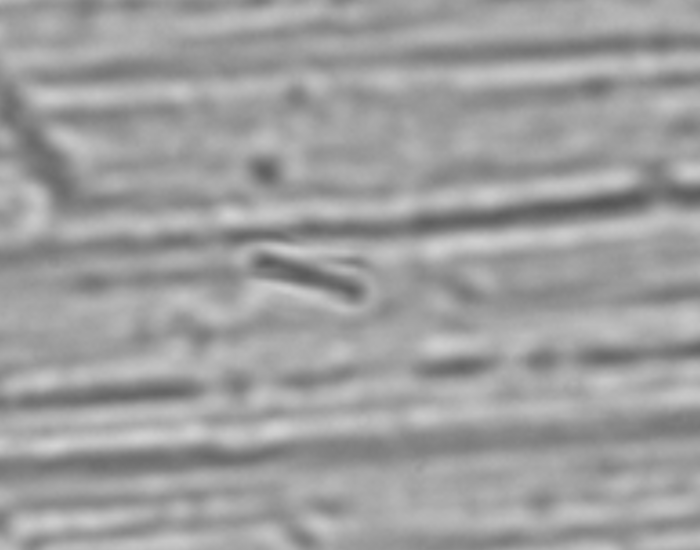
\includegraphics[width=\textwidth]{figures/improvements/unpolished.png}
 \caption{An unusually severe case of the PDMS ridges creating noise.}\label{fig:unpolished}
 \end{subfigure}\hspace{1em}%
 \begin{subfigure}[3b]{0.40\textwidth}
 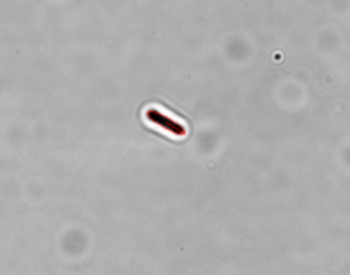
\includegraphics[width=\textwidth]{figures/improvements/polished.png}
 \caption{After being polished there is no trace of ridges in the PDMS.}\label{fig:polished}
 \end{subfigure}
 \caption{The effects of polishing the channel using emery cloth and a silicate abrasive. (a) Shows sharp lines along the length of the channel disturbing tracking, (b) no ridges can be seen.}
 \label{fig:polisheffect}
 \end{figure}

To solve this the copper mold in which the PDMS channels are formed was polished with a silicate abrasive (Autosol) and emery cloth. This removed all visible scratches from the mold and therefore from the PDMS, as seen in Figure \ref{fig:polished}.